\section{Flash storage and filesystems}

\begin{frame}
  \frametitle{Block devices vs raw flash devices: reminder}
  \begin{itemize}
  \item Block devices:
    \begin{itemize}
    \item Allow for random data access using fixed size blocks
    \item Do not require special care when writing on the media
    \item Block size is relatively small (minimum 512 bytes, can be
      increased for performance reasons)
    \item Considered as reliable (if the storage media is not, some
      hardware or software parts are supposed to make it reliable)
    \end{itemize}
  \item Raw flash devices:
    \begin{itemize}
    \item Flash chips directly driven by the flash controller on your SoC.
          You can control how they are managed.
    \item Allow for random data access too, but require erasing before
          writing on the media.
    \item Read and write block size (for example 4 KiB) don't use
          the same block size as erasing (for example 128 KiB).
    \item Multiple flash technologies: NOR flash, NAND
          flash (Single Level Cell - SLC: 1 bit per cell, MLC: multiple bits per cell).
    \end{itemize}
  \end{itemize}
\end{frame}

\begin{frame}[fragile]
  \frametitle{NAND flash storage: constraints}
  \begin{columns}
  \small
  \column{0.7\textwidth}
  \small
  \begin{itemize}
  \item Reliability
    \begin{itemize}
    \item Reliability depends on flash technology (SLC, MLC)
    \item Require mechanisms to recover from bit flips: ECC (Error
          Correcting Code), stored in the OOB (Out-Of-Band area)
    \end{itemize}
  \item Lifetime
    \begin{itemize}
    \item Relatively short lifetime: between 1,000,000 (SLC) and 1,000
          (MLC) erase cycles per block
    \item Wear leveling required to erase blocks evenly
    \item Bad block detection/handling required too
    \end{itemize}
  \item Widely used anyway in embedded systems for several reasons:
        low cost, high capacity, good read and write performance.
  \end{itemize}
  \column{0.3\textwidth}
  \includegraphics[width=\textwidth]{slides/sysdev-flash-filesystems/nand-organization.pdf}
  \end{columns}
\end{frame}

\begin{frame}
  \frametitle{The MTD subsystem}
  \begin{columns}
  \column{0.5\textwidth}
  \begin{itemize}
  \item MTD stands for {\em Memory Technology Devices}
  \item Generic subsystem in Linux dealing with all types of storage media that
        are not fitting in the block subsystem
  \item Supported media types: RAM, ROM, NOR flash, NAND flash,
        Dataflash...
  \item Independent of the communication interface (drivers available
        for parallel, SPI, direct memory mapping, ...)
  \item Abstract storage media characteristics and provide a simple
        API to access MTD devices
  \end{itemize}
  \column{0.5\textwidth}
    \includegraphics[width=\textwidth]{slides/sysdev-flash-filesystems/mtd-architecture.pdf}
  \end{columns}
\end{frame}

\begin{frame}
  \frametitle{MTD partitioning}
  \begin{itemize}
  \item MTD devices are usually partitioned
    \begin{itemize}
    \item It allows to use different areas of the flash for different
      purposes: read-only filesystem, read-write filesystem, backup
      areas, bootloader area, kernel area, etc.
    \end{itemize}
  \item Unlike block devices, which contains their own partition
    table, the partitioning of MTD devices is described externally
    (don't want to put it in a flash sector which could become bad)
    \begin{itemize}
    \item Specified in the board Device Tree (default partitions, not always relevant)
    \item Specified through the kernel command line
    \end{itemize}
  \item Each partition becomes a separate MTD device
    \begin{itemize}
    \item Different from block device labeling (\code{sda3},
      \code{mmcblk0p2})
    \item \code{/dev/mtd1} is the second enumerated partition on the
      system (either from a single flash chip or from a different one).
    \item Note that the master MTD device (the device those partitions
      belong to) is not exposed in \code{/dev}
    \end{itemize}
  \end{itemize}
\end{frame}

\begin{frame}[fragile]
  \frametitle{Defining MTD partitions}
  \scriptsize
  \begin{itemize}
  \item MTD partitions must start and end at erase block boundaries
  \item MTD partitions are defined through the kernel command line. Example:\\
        \code{mtdparts=omap2-nand.0:512k(XLoader)ro,1536k(UBoot)ro,512k(Env),4m(Kernel),-(Root)}\\
	(\code{omap2-nand.0} is the NAND device name for Linux, check the boot log)
  \item U-Boot understands the Linux syntax:
  \begin{verbatim}
# Association between flash device U-Boot name (nand info) and Linux name
setenv mtdids nand0=omap2-nand.0
# Partition definitions
setenv mtdparts mtdparts=omap2-nand.0:512k(XLoader)ro,1536k(UBoot)ro...
  \end{verbatim}
  \end{itemize}
  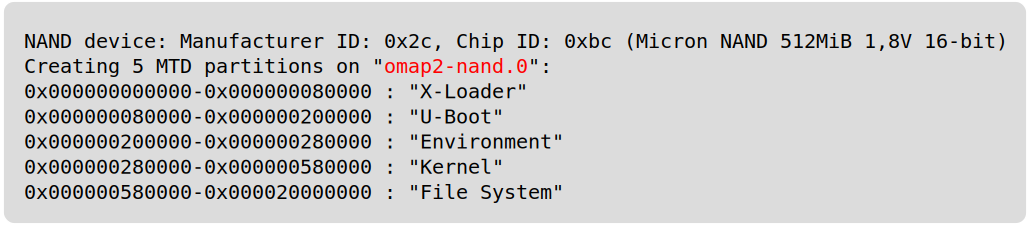
\includegraphics[height=0.35\textheight]{slides/sysdev-flash-filesystems/kernel-mtd-log.pdf}
\end{frame}

\begin{frame}[fragile]
  \frametitle{Commands to manage NAND devices}
  \begin{itemize}
  \item From U-Boot
     \begin{itemize}
     \item \code{help nand} to see all \code{nand} subcommands
     \item \code{nand info}, \code{nand read}, \code{nand write}, \code{nand erase}...
     \end{itemize}
  \item From Linux
     \begin{itemize}
     \item {\bf mtdchar} driver: one \code{/dev/mtdX} and \code{/dev/mtdXro}
           character device per partition.
     \item Accessed through \code{ioctl()} operations to erase and flash
	   the storage.
     \item Used by these utilities: \code{flash_eraseall}, \code{nandwrite}\\
           Provided by the {\em mtd-utils} package, also available in BusyBox
     \item There are also host commands in {\em mtd-utils}: \code{mkfs.jffs2}, \code{mkfs.ubifs}, \code{ubinize}...
     \end{itemize}
  \end{itemize}
\end{frame}

\begin{frame}
  \frametitle{Flash wear leveling}
  \begin{itemize}
  \item Wear leveling consists in distributing erases over the whole
    flash device to avoid quickly reaching the maximum number of erase
    cycles on blocks that are written really often
  \item Can be done in:
    \begin{itemize}
    \item the filesystem layer (JFFS2, YAFFS2, ...)
    \item an intermediate layer dedicated to wear leveling (UBI)
    \end{itemize}
  \item The wear leveling implementation is what makes your flash
    lifetime good or not
  \end{itemize}
\end{frame}

\begin{frame}
  \frametitle{Flash file-systems}
  \begin{itemize}
  \item 'Standard' file systems ({\em ext2}, {\em ext4}...) are
        meant to work on block devices
  \item Specific file systems have been developed to deal with
        flash constraints
  \item These file systems are relying on the MTD layer to access
    flash chips
  \item There are several legacy flash filesystems which might be
    useful for small partitions: JFFS2, YAFFS2.
  \item Nowadays, UBI/UBIFS is the de facto standard for medium to
    large capacity NANDs
  \end{itemize}
\end{frame}

\begin{frame}
  \frametitle{UBI (1)}
  \begin{columns}
    \column{0.7\textwidth}
    {\em UBI: Unsorted Block Images}
    \begin{itemize}
    \item Design choices:
      \begin{itemize}
      \item Split the wear leveling and filesystem layers
      \item Add some flexibility
      \item Focus on scalability, performance and reliability
      \end{itemize}
    \item Drawback: introduces noticeable space overhead,
          especially when used on small devices or partitions. JFFS2
          still makes sense on small MTD partitions.
    \item Implements logical volumes on top of MTD devices
          (like LVM for block devices)
    \item Allows wear leveling to operate on the whole storage,
	  not only on individual partitions.
    \end{itemize}
    \url{http://www.linux-mtd.infradead.org/doc/ubi.html}
    \column{0.3\textwidth}
    \includegraphics[height=0.8\textheight]{slides/sysdev-flash-filesystems/ubifs.pdf}
  \end{columns}
\end{frame}

\begin{frame}
  \frametitle{UBI (2)}
  \begin{center}
    \includegraphics[width=\textwidth]{slides/sysdev-flash-filesystems/ubi.pdf}
  \end{center}
  When there is too much activity on an LEB, UBI can decide to move it
  to another PEB with a lower erase count. Even read-only volumes
  participate to wear leveling!
\end{frame}

\begin{frame}
  \frametitle{UBI: good practice}
  \begin{itemize}
  \item UBI distributes erases all over the flash device: the more space
    you assign to a partition attached to the UBI layer the more efficient
    wear leveling will be.
  \item If you need partitioning, use UBI volumes, not MTD partitions.
  \item Some partitions will still have to be MTD partitions: e.g. the
    bootloaders.
  \item U-Boot now even supports storing its environment in a UBI volume!
  \item If you do need extra MTD partitions, try to group them at the
    beginning of the flash device (often more reliable area).
  \end{itemize}
  \includegraphics[height=0.3\textheight]{slides/sysdev-flash-filesystems/ubifs-bad-layout.pdf}
  \hfill
  \includegraphics[height=0.3\textheight]{slides/sysdev-flash-filesystems/ubifs-good-layout.pdf}
\end{frame}

\begin{frame}
  \frametitle{UBIFS}
  {\em Unsorted Block Images File System}
  \begin{itemize}
  \item \url{http://www.linux-mtd.infradead.org/doc/ubifs.html}
  \item Journaling file system providing better performance than
        its predecessor (JFFS2) and addressing its scalability issues
  \item UBIFS filesystem images can be created using \code{mkfs.ubifs}
        from {\em mtd-utils}:\\
      \code{mkfs.ubifs -m 4096 -e 258048 -c 1000 -r rootfs/ ubifs.img}
      \begin{itemize}
      \item \code{-m 4096}: minimal I/O size\\
                 (see \code{/sys/class/mtd/mtdx/writesize}).
      \item \code{-e 258048}: {\bf logical} erase block size (smaller than
                 PEB size, can be found in the kernel log after running
		 \code{ubiattach})
      \item \code{-c 1000}; maximum number of erase blocks for the
        UBI volume the image will be flashed into. A pessimistic
	number will increase metadata size and degrade performance.
      \end{itemize}
  \item This image can then be flashed on a volume\\
        or included in a UBI image (\code{ubinize} command).
  \end{itemize}
\end{frame}

\begin{frame}[fragile]
  \frametitle{ubinize: create a UBI image}
  \small
  \begin{itemize}
  \item \code{ubinize} creates a UBI image to be flashed on an MTD partition,
	from a specification of the contents of its volumes.
  \item \code{static} volumes are meant to store {\bf read-only} blobs of data,
	and get the minimum corresponding size. CRC checks are done on
        them.
  \item A read-only UBIFS filesystem can go in a \code{static}
	volume, but in this case \code{dynamic} volumes are best
        for performance (CRC checking also done at UBIFS level).
  \item \code{autoresize}: allows to fill all remaining UBI space
  \item Example configuration file for \code{ubinize}:
  \end{itemize}
  \begin{columns}
\column{0.33\textwidth}
\scriptsize
\begin{verbatim}
[kernel-volume]
mode=ubi
image=zImage
vol_id=1
vol_type=static
vol_name=kernel
\end{verbatim}
\column{0.33\textwidth}
\scriptsize
\begin{verbatim}
[rootfs-volume]
mode=ubi
image=rootfs.ubifs
vol_id=2
vol_size=2MiB
vol_type=dynamic
vol_name=rootfs
\end{verbatim}
\column{0.33\textwidth}
\scriptsize
\begin{verbatim}
[data-volume]
mode=ubi
image=data.ubifs
vol_id=3
vol_size=30MiB
vol_type=dynamic
vol_name=data
vol_flags=autoresize
\end{verbatim}
  \end{columns}
\end{frame}

\begin{frame}
  \frametitle{ubinize command line}
  \begin{itemize}
  \item \code{ubinize} takes the following arguments:
    \begin{itemize}
    \item \code{-o <output-file-path>}\\
	Path to the output image file
    \item \code{-p <peb-size>}\\
	The PEB size (MTD erase block size)
    \item \code{-m <min-io-size>}\\
	The minimum write unit size (MTD write size)
    \item \code{-s <subpage-size>}\\
	Subpage size, only needed if both your flash and your
	flash controller are supporting subpage writes
    \item The last argument is the path to the \code{ubinize}
	  configuration file
    \end{itemize}
  \item Example: \code{ubinize -o ubi.img -p 256KiB -m 4096 -s 2048 ubinize.cfg}
  \end{itemize}
\end{frame}

\begin{frame}
  \frametitle{Linux: UBI image creation workflow}
  \begin{center}
    \includegraphics[scale=0.3]{slides/sysdev-flash-filesystems/ubi-creation-workflow.pdf}
  \end{center}
\end{frame}

\begin{frame}{U-Boot: main UBI commands}
  Grouped under the \code{ubi} command
    \begin{itemize}
    \item \code{ubi part <part-name>}\\
	Attach an MTD partition to the UBI layer. Example:\\
	\code{ubi part UBI}
    \item \code{ubi readvol <dest-addr> <vol-name> [<size>]}\\
	Read volume contents. Example:\\
	\code{ubi readvol 0x21000000 kernel}
    \item \code{ubi writevol <src-addr> <vol-name> <size>}\\
        Write to volume. Example:\\
	\code{tftp 0x21000000 data.ubifs}\\
	\code{ubi writevol 0x21000000 data ${filesize}}
    \end{itemize}
\end{frame}

\begin{frame}{U-Boot: UBIFS commands}
  U-Boot also has commands to access UBIFS partitions:
    \begin{itemize}
    \item \code{ubifsmount ubi<n>:<volume-name>}\\
	Mount the specified volume. Example:\\
        \code{ubifsmount ubi0:root}
    \item \code{ubifsload <addr> <filename> [bytes]}\\
	Load file contents at the specified address. Example:\\
	\code{ubifsload 0x21000000 boot/zImage}
    \item Other commands: \code{ubifsls} and \code{ubifsumount}
    \end{itemize}
    This shows that to optimize space, the kernel and DTB can
    also be stored in a UBIFS partition. Otherwise, the DTB volume
    consumes an entire LEB.
\end{frame}

\begin{frame}
  \frametitle{Linux: UBI / UBIFS target tools}
  \begin{itemize}
  \item Target tools exist for creating UBI spaces and manipulating volumes:\\
    see \url{http://www.linux-mtd.infradead.org/doc/ubi.html\#L_usptools}
  \item Attaching a MTD partition to UBI:\\
    \code{ubiattach -m <MTD-device-id> /dev/ubi_ctrl}
  \item Commands to manipulate volumes:\\ \code{ubimkvol},
    \code{ubirmvol}, \code{ubiupdatevol}, \code{ubirsvol},
    \code{ubirename}
  \item Mounting a UBIFS filesystem:\\
    \code{mount -t ubifs <ubi-device-id>:<volume-name> <mount-point>}
  \item Example:\\
    \code{mount -t ubifs ubi0:data /data}
  \end{itemize}
\end{frame}

\begin{frame}
  \frametitle{Linux: Using a UBIFS filesystem as root filesystem}
  \begin{itemize}
  \item You just have to pass the following information on the kernel
    command line:
    \begin{itemize}
    \item \code{ubi.mtd=UBI}\\
      Attach the MTD partition named \code{UBI} to the UBI layer and
      create \code{ubi0}.\\
      Note: you can also use the MTD partition number (more error
      prone): \code{ubi.mtd=1}
    \item \code{rootfstype=ubifs root=ubi0:rootfs}\\
      Mount the \code{rootfs} volume on \code{ubi0} as a UBIFS filesystem
    \item \code{rootfstype=} lets the kernel know what filesystem
      to mount as root filesystem. It's mandatory for UBIFS, but
      it can also be used for block filesystems. This way the kernel
      doesn't have to try all the filesystems it supports. This reduces
      boot time.
    \end{itemize}
  \item Example: \code{rootfstype=ubifs ubi.mtd=UBI root=ubi0:rootfs}
  \end{itemize}
\end{frame}

\begin{frame}
  \frametitle{Linux: Block emulation layers}
  \begin{itemize}
  \item Sometimes needed to use read-only block filesystems such as Squashfs and EROFS
  \item Linux provides two block emulation layers:
    \begin{itemize}
    \item \code{mtdblock} (\kconfig{CONFIG_MTD_BLOCK}):
       block devices emulated on top of MTD devices.
       \begin{itemize}
       \item Named \code{/dev/mtdblockX}, one for each partition.
       \item Originally the \code{mount} wanted a block device to mount JFFS2 and YAFFS2.
       \item Don't write to \code{mtdblock} devices: bad blocks are not handled!
       \end{itemize}
    \item \code{ubiblock} (\kconfig{CONFIG_MTD_UBI_BLOCK}):
       {\bf read-only} block devices emulated on top of UBI volumes
       \begin{itemize}
       \item Used on static (read-only) volumes
       \item Usually named \code{/dev/ubiblockX_Y}, where X is the UBI device
             id and Y is the UBI volume id (example: \code{/dev/ubiblock0_3})
       \end{itemize}
    \end{itemize}
  \end{itemize}
\end{frame}
